%Préambule
\documentclass[12pt]{report}

\usepackage[french]{babel}
\usepackage{luatextra}
\usepackage{hyperref}
\usepackage{hhline}
\usepackage{multirow}
\usepackage{listings}
\usepackage{caption}
\usepackage{amsmath}
\usepackage{enumitem} % listes à puces

\usepackage{lastpage}

\usepackage{fancyhdr}


\pagestyle{fancy}

\renewcommand{\thesection}{\Roman{section}}

%Information sur le document
\title{Projet d'Algorithmique \\ \textit{L'Ascenseur} }
\date{Mai-juin 2019}
\author{Victor \textsc{ALAIN} - Arthur \textsc{BLAISE} - Amélie \textsc{GUEDES} \\ - Loann \textsc{POTTIER}}

 \makeatletter
\let\theauthor\@author
\let\thetitle\@title
\let\thedate\@date
\makeatother

%En-tête
\fancyhead[L]{}
\fancyhead[C]{\rightmark}
\fancyhead[R]{}

%Pied-de-Page
\fancyfoot[L]{\thedate}
\fancyfoot[C]{\thepage\ / \pageref{LastPage}}
\fancyfoot[R]{\thetitle}

%Refonte du style des sections
\usepackage{titlesec}
\titleformat{\section}[display]
  {\normalfont\huge\bfseries\sffamily}
  {}
  {-15pt}
  {\LARGE}

\begin{document}

\renewcommand{\thesection}{\textbf{\Roman{section}}} % Supprimer les numéros de chapitres dans la table des matières

\maketitle
\tableofcontents

\clearpage


\section{Introduction}

\subsection{Avant-propos}
	Le jeu de l'ascenseur est un jeu de cartes complexe qui nécessite, pour y jouer, de bien maîtriser les règles. Pour reproduire ce jeu il nous fallait donc évidemment savoir y jouer, c'est dans ce but que nous avons essayé de synthétiser les règles essentielles à la création de l'algorithme. L'une des difficultés majeures a sans doute été la distribution des points à la fin de chaque manche, ou le listage des cartes qu'il est possible de jouer.\\
	
	Mais au final, cette partie réelle nous a permis de relever les points importants, et d'avoir une schématisation plus concrète du déroulement du jeu. Nous avons essayé de résumer les étapes principales du développement ici.

	
\subsection{Problèmes à résoudre}
	
	Le but de ce projet est de réaliser un algorithme permettant d'exécuter le jeu de l'Ascenseur. Voici la liste des problématiques qui se sont présentées :\\
	
	\begin{itemize}[label=\textbullet, font=\LARGE]
		\item La première partie concerne la configuration du jeu : en effet il existe plusieurs variantes des règles, comme le nombre de joueurs, ou le nombre de points gagnés par manche... Il nous faut donc trouver un moyen pour laisser aux joueurs la possibilité de les modifier.
		
		Ce moyen a pris la forme d'un fichier config.txt qui résume sept options différentes : le nombre maximal de joueurs (humains et bots), le nombre de points gagnés par défaut à une manche remportée, le nombre de points gagnés ou perdu par pli, la taille en pixels de la fenêtre de jeu, et les limites d'âge des joueurs (qui sont demandées pour départager les joueurs).\\
		
		\item Ensuite vient le développement d'une partie : gérer le nombre de manches par phase (qui varie en fonction du nombre de joueurs), le nombre de tours par manche, la distribution ou la remise des cartes... à ce stade même la question de qui doit recevoir ses cartes en premier semble complexe.
		
		Lors d'une manche il faut aussi compter le nombre de plis remportés par chaque joueur, sans oublier de lui demander son pari au début. De surcroît chaque joueur ayant remporté une manche doit débuter la manche suivante. Il est important également de contrôler quelle carte chaque personne joue, pour vérifier que la couleur soit bien valide. Chaque joueur joue une carte de la couleur demandée s'il en possède une, sinon il doit jouer un atout. Cependant, un joueur n'est pas obligé de poser un atout s'il n'a pas de carte de la même couleur, il peut déposer une carte quelconque mais il perdra le tour. Il est aussi à noter que les jokers n'ont pas été inclus dans le jeu.\\
		
		\item La fin de la partie est heureusement simple à créer : le joueur ayant le plus de points gagne, point final.\\

		\item En annexe, une autre partie de code est ajoutée : la gestion des bots. Maintenant que les humains peuvent jouer, il faut leur permettre de jouer contre un ordinateur. C'est une partie assez ardue à modéliser puisqu'il faut prévoir plusieurs 'personnalités' d'Intelligence Artificielle, et créer l'algorithme correspondant.
	\end{itemize}
	
	\begin{figure}[h]
	\centering
	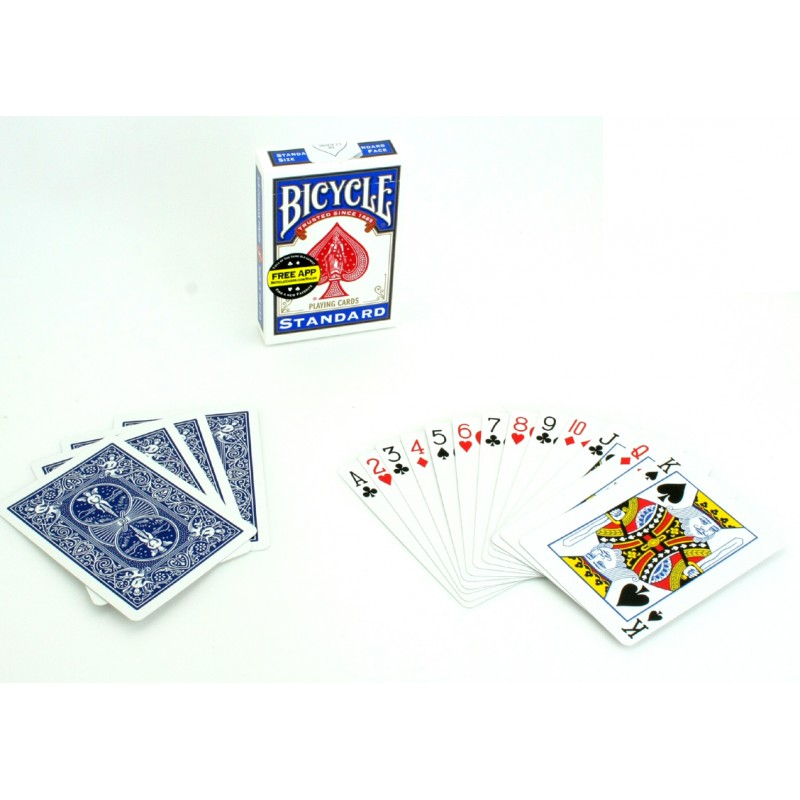
\includegraphics[scale=0.25]{jeu-de-cartes.jpg}
	 \caption{Jeu de carte utilisé lors d'une partie d'ascenseur}
	\end{figure}
		

		
\clearpage

		
\section{Explication des algorithmes}
Pour commencer, voici comment est construit le code. Tout part d'un programme principal \textit{start.pas} : c'est ce programme qui lance toutes les fonctions secondaires et les appellent dans le bon ordre, afin de permettre le bon déroulement du jeu. De surcroît ce programme utilise des unités, chacune s'occupant d'une partie spécifique du jeu.
  	\subsection{Structure du programme}
  
   \subsubsection{Programme principal}
   Le programme principal \textit{projet2.pas} demande à chaque joueur de renseigner son pseudo et son âge, qui seront utilisés dans le reste de la partie. Dans ce programme il y a également l'utilisation des \textit{unités}, ce qui évite d'avoir un fichier trop long (en segmentant le code, il devient plus lisible, et plus facile à tester). \\
   
   Ensuite, durant le déroulement du programme les choses se complexifient car le déroulement du jeu est définit dans deux unités. L'une demande si le joueur souhaite afficher les règles (unit \textit{intro.pas}), et l'autre contient chaque étapes du jeu (unit \textit{deroulement.pas}). Cette dernière utilise l'unité \textit{bot.pas} pour intégrer des Intelligences artificielles au jeu. \\
   
 Afin d'assurer le déroulement visuel du jeu l'aspect graphique est contenu dans une autre unité : \textit{graph.pas}. Celle-ci fonctionne un peu comme une lib graphique spécialement conçue pour le jeu de l'Ascenseur, en appelant d'elle même les unités gLib2D, SDL et autres. Le fait de l'avoir concentrée en un seul fichier permet de ne pas avoir trop d'appels ou d'import dans le reste du code. Dans ce même but, l'unité \textit{classes.pas} rassemble toutes les classes utilisées dans le jeu.
 \clearpage
   
   \subsection{Unités utilisées}

   	\subsubsection{\cdot ~Unité Intro}
   	Cette unité est particulièrement simple car elle se contente de proposer à l'utilisateur la lecture des règles du jeu. Rapide et efficace.
   	
	\subsubsection{\cdot ~Unité deroulement}
 Cette unité est initialement le cœur du programme; elle fait donc appel à 11 fonctions et 9 procédures différentes. Ces dernières sont : \\
  \begin{description}
 \item[InitJoueur:] Demande le nombre de joueurs présent dans la partie
 \item[InitPliManche:] Permet de ramener le nombre de plis des joueurs à zéro avant la nouvelle manche
 \item[Inarray:] Vérifie la présence d'une carte dans la liste
 \item[Init:] Créé le paquet de carte
 \item[distribuer:] Distribue les cartes aux joueurs et empêche le doublon de carte
\item[Parions:] Enregistre le pari d’un joueur en prenant en compte les contrainte de jeu 
\item[PlusJeune:] Change l’ordre de la liste avec le plus jeune joueur en premier
 \item[InitAtout:] Permet d'initialiser la couleur de la carte de l'atout
\item[VerifAtout:] Vérifie que la carte atout n’est pas dans un paquet de joueur
 \item[NombreManche:] Calcul le nombre de manches nécessaires vis-à-vis du nombre de joueur
 \item[VerifDroitDePoser:] Vérifie si la cartes peut-être poser sans enfreindre les règles
 \item[BestPli:] A la fin d'un tour, renvoie un entier pour désigner le gagnant
 \item[RetirePaquet:] Retire la carte du paquet une fois sélectionner
 \item[OrdreJoueur:] Permet de déterminer et d'appliquer l'ordre de jeu des joueurs pour le prochain pli
 \item[ComptageDePoint:] Compte le nombre de point associé aux joueurs
 \item[creerjoueur:] Prend le pseudo et l’âge d’un joueur, et l’enregistre comme non bot pour simplifier son utilisation dans le programme
\item[creerjoueurs:] Réitère la fonction précédente pour enregistrer tous les joueurs
 \end{description}
  \vspace{15pt}
  
  \subsubsection{\cdot ~Unité graph}
	
	C'est le morceau de code qui permet de gérer toute l'interface graphique : de l'affichage du fond d'écran jusqu'au clic sur une carte, en passant par la saisie des paris ou les animations discrètes, tout est géré ici puis appelé dans le programme.  
  
  \begin{description}
  	\item[init:] Initialise la fenêtre avec une taille, et crée la référence de l'image de fond
  	\item[set\_deck:] Initialise la liste des cartes présentes dans le deck
  	\item[set\_cartes\_main:] Définit les cartes dans les mains du joueur
  	\item[set\_joueur:] Définit le joueur qui doit être affiché en focus (indicateur en haut à gauche de la fenêtre)
  	\item[set\_fps:] Initialise le nombre d'images par seconde
	\item[convert\_carte:] Complète les informations d'une carte pour la rendre utilisable par la lib graphique
	\item[load\_players:] Complète les informations d'un joueur pour le rendre utilisable par la lib graphique
	\item[convert\_text:] Convertit un texte en élément graphique
	\item[convert\_couleur] Convertit une couleur en bits (utilisé par le terminal) en une couleur graphique
	\item[afficher\_cartes]: Affiche la liste de cartes définie par \textit{set\_deck}
	\item[afficher\_joueurs:] Affiche la liste des joueurs autours de la "table"
	\item[afficher\_background:] Affiche l'image de fond
	\item[afficher\_texte:] Affiche un message
	\item[refresh:] Rafraîchit l'affichage de la fenêtre
	\item[focus\_joueur:] Affiche le pseudo du joueur focus en haut à gauche de l'écran
	\item[afficher\_atout:] Affiche la couleur de l'atout actuel
	\item[afficher\_manche:] Affiche la liste des cartes définies par \textit{set\_main}
	\item[afficher\_cadre:] Affiche un cadre autour de la carte survolée par la souris 
	\item[on\_click:] Retourne la carte où le joueur a cliqué
	\item[saisir\_txt:] Demande à l'utilisateur de saisir du texte
	\item[afficher\_score:] Affiche le score des joueurs dans une zone blanche, au milieu de la fenêtre
  \end{description}
  \vspace{15pt}

\subsubsection{\cdot ~Unité bot}
	Cette partie du programme permet de modéliser une intelligence artificielle pour le jeu Ascenseur. Elle est constituée de: \\
\begin{description}
  	\item[CreerBot:] Permet de créer les bots avec leurs age et leurs pseudos
	\item[PartieBot:] Demande le nombre d'IA souhaité
	\item[ChoixCarteCouleurBot:] Affiche une carte d'une couleur de L'IA en fonction de la carte jouée précédemment
	\item[ChoixCarteBotPrems:] Affiche une carte aléatoire quand l'IA commence à jouer le pli	
\end{description}

\clearpage

\section{Difficultés}
	\subsection{Cœur du programme}
	La principale difficulté rencontrée fût dans le choix des fonctions à réaliser mais surtout comment réaliser certaines fonctions. De plus, une autre difficulté était au moment de relié notre unit à l'interface graphique car les données entre les deux programmes étaient relativement différente. Nous avons également eu du mal à démarrer car les règles énoncés n'étaient pas très claires et nous avions tous compris des règles différentes, surtout au niveau du comptage des points.
	
	\subsection{Unité graphique}
	La principale difficulté rencontrée lorsque nous avons commencé la partie graphique est l'installation : malgré de nombreuses heures de tests, il nous a été impossible d'utiliser la lib SDL sur nos ordinateurs personnels. Cela nous a donc forcé à la travailler uniquement depuis les postes de l'école, ralentissant la progression de cette section du programme.\\ 
	
	D'autres problèmes sont apparus au fur et à mesure du code : par exemple il fallait pouvoir modifier la taille de la fenêtre afin de l'adapter à la taille de l'écran, ce que ne proposait pas nativement gLib2D. Nous avons donc dû modifier cette unité pour ajouter une fonction qui modifie l'échelle de la fenêtre, elle-même appelée par la procédure \textit{init}. \\

	Certains défis se sont révélés intéressants à relever. Comment afficher les 52 cartes différentes sans avoir à les sauvegarder une par une sous forme d'image ? Nous avons opté pour la formation d'un rectangle blanc avec du texte superposé pour afficher la valeur et la couleur. Comment afficher les cartes, joueurs et autres items plus de 50 fois par seconde sans mettre à plat la mémoire libre de l'ordinateur ? Ils sont générés une seule fois puis stockés dans une variable de l'unité. Comment demander à l'utilisateur de saisir du texte ? Nous affichons une sous-fenêtre invitant l'utilisateur à écrire, puis on interrompt le programme afin de détecter les clics sur le clavier et afficher le résultat en temps réel. Et encore bien d'autres...

\vspace{15pt}

\subsection{Raccordement}
	On parle du raccordement lorsque l'on rassemble la partie graphique de la partie déroulement de la partie. Pour ce faire, nous avons changé plusieurs fonctions et écrit un algorithme principal. \\
La plus grande difficultée fût la manière de réfléchir. En effet, nous avions rédigés l’unité déroulement.pas comme un ensemble de fonctions et procédures s’appelant les unes les autres pour faire une partie. Cependant, pour ajouter la partie graphique, il fallait une structure différente avec une boucle while et appeler les fonctions et procédures avec des conditionnelles pour faire jouer une partie. Cela nous a pris beaucoup de temps car on ne l’avait encore jamais fait. \\
 
\clearpage

\section{Avantages et limites}
\paragraph{} Notre algorithme comporte de nombreux avantages et inconvénients. Au niveau des désavantages, nous n’avons malheureusement pas réussi à tester notre programme puisque nous n’avons pas pu être à l’EISTI après avoir fini le programme et l’exécution que nous avons faite n’a pas marchée. Cependant, nous avons pu nous assurer que notre programme compile. \\
\paragraph{} De plus, notre programme ne fonctionne que sur un seul ordinateur, c’est-à-dire qu’il est impossible pour les joueurs de jouer en ligne. Nous aurions aimé mettre en place cette option. Néanmoins, par manque de temps et de base technique sur le sujet, nous n’avons pas pu. \\
\paragraph{} En terme d’avantages, notre programme est bien structuré, bien commenté, et même si nous n’avons pas pu vérifier, devrait fonctionner normalement. De plus, nous avons beaucoup appris lors de ce projet. En effet, il nous a permis de consolider nos bases que ce soit sur les fonctions ou même les procédures et de découvrir de nouvelles fonctionnalités comme la lib graphique. \\
\paragraph{} De plus, Arthur a travaillé l’interface pour qu’elle soit agréable à utiliser. En effet, le choix des couleurs est simple, les cartes sont basiques (on n’a pas téléchargé de jeu de cartes, on a créé les cartes) mais l’utilisation est simple. Et enfin, l’interface se suffit à elle-même. En effet, on a très peu besoin du terminal.

\clearpage
\section{Contribution des étudiants}
\subsection*{Arthur Blaise}
	Arthur s'est concentré sur l'utilisation de l'unité gLib2D, et la création de la lib graphique, pour pouvoir l'implémenter plus tard dans le programme. En annexe, il y a aussi eu la gestion du fichier de configuration.
	
\subsection*{Amélie Guédès et Victor Alain}
 Amélie et Victor se sont occupés du plus important, le cœur du programme. De la création des joueurs à la fin de la partie, en passant par le déroulé de chaque manche, chaque pli. 
 
\subsection*{Loann Pottier}
Loann a rejoint le projet en cours de route et, faute de pouvoir coder, s'est appliqué à comprendre le programme pour le résumer dans ce rapport.


\clearpage
\section{Bilan personnel}
\subsection{Amélie Guédès}
En ce qui me concerne, j'ai trouvé ce projet intéressant. On a eu une bonne cohésion de groupe, ce qui a permis un travail efficace. Il y a eu des passages difficiles comme le moment où l’on a dû reprendre la moitié de l'unité \textit{deroulement} pour s'adapter à la partie graphisme. J'ai beaucoup appris, notamment qu'il faut toujours voir un programme sous plusieurs angles afin de mieux s'adapter aux contraintes. A partir du moment où l'on a eu une vision d'ensemble du programme, il a été beaucoup plus simple de l'adapter au graphisme, et ainsi adapter la façon de changer de pli par exemple. On est passé d'une fonction \textit{pli} qui prenait les cartes que chaque joueur jouait et renvoyait le numéro du joueur remportant le pli, à une conditionnelle dans le programme principal qui nous permet de savoir quand on change de pli avec une variable p quand le dernier joueur a joué. Cette manière de structurer était indispensable pour revenir au début de la boucle while à chaque changement de joueur et ainsi rafraîchir régulièrement l'interface graphique.

\vspace{15pt}

\subsection{Arthur Blaise}
Pour ma part, j'ai beau avoir une certaine expérience de la programmation, ce projet a été mon premier vrai travail avec une interface graphique. J'ai pu découvrir le monde du SQL, la gestion des événements, l'utilisation du cache pour limiter les fuites de mémoire, et plein d'autres choses passionnantes. Même si j'ai passé de longues heures à m'arracher les cheveux sur des problèmes d'apparence simples et à pester contre Pascal, je n'en reste pas moins fier du travail accompli. Ce jeu est tellement complexe à modéliser, sans même parler de l'affichage, que notre programme valait la peine d'être créé. Et tant pis pour les longues heures nocturnes derrière mon ordinateur...

\vspace{15pt}

\subsection{Victor Alain}

De mon côté, ce projet m'a permis comme le précédent à m'améliorer en algorithmique, à penser différemment, à découvrir de nouvelles fonctionnalités. J'ai également appris comment départagé des algorithmes, c'est-à-dire à quel moment il faut faire plusieurs fonctions ... De plus, travailler en binôme à été bénéfique pour mieux comprendre les différents fonction ou procédures, mais également pour corriger les fautes que l'on pouvaient faire. Notre méthode de travail a également été différente et je ne fonctionnais pas comme cela auparavant. En effet, nous avons commencé par la procédure de fin et nous avons finis par la première fonction.

\vspace{15pt}

\subsection{Pottier Loann}

Ce projet fut intéressant car il m'a permis d'observer l'utilisation et le codage d'une interface graphique. Cependant, le temps manquait pour faire le programme le plus optimisé possible. Ce dernier reste tout de même correct. L'interface graphique fut long à coder mais pas la plus difficile; en effet, le raccordement au programme principal de cette dernière fut plus complexe. Dans ma partie de la rédaction du rapport, la difficulté n'était pas présente et j'ai pu le rédiger efficacement grâce à la communication au sein du groupe. Mes camarades ont également accepté de faire une relecture qui m'a bien aidée.
\clearpage
\section{Conclusion}

	Pour conclure, plus de temps nous aurait sûrement permis d’améliorer encore notre programme. Mais dans l’ensemble, nous sommes fiers du résultat. Même si nous n'avons pas eu l'occasion de tester à cause de ces problèmes matériels, dans la théorie, l'interface est belle et travaillée, avec un côté moderne qui change du style habituel du tapis vert, et une communication avec les utilisateurs facile. De plus, le code interne est fonctionnel, ce qui permet une assez grande modularité. Les bots sont sympathiques, et l'ensemble a été longuement travaillé et retravaillé jusqu'à obtenir un résultat optimal. Donc même si finalement tout ne fonctionnerait pas comme prévu, au moins nous avons appris beaucoup de choses et sommes fiers du travail accompli !
			
\end{document}
